\documentclass{article}
\title{Misura della costante di gravitazione universale\\tramite un pendolo di torsione}
\author{Lorenzo Redighieri\\Federico Tronchi\\Luca Zoppetti}
\date{26 Maggio 2023}

\usepackage{graphicx}
\usepackage[margin=100pt]{geometry}

\usepackage{float}
\usepackage{textcomp, gensymb}
\usepackage{amssymb}
\usepackage{amsmath}
\usepackage{cite}
\usepackage{tikz}

\usepackage[italian]{babel}

\newcommand{\quotes}[1]{``#1''}
\newcommand{\abs}[1]{\left| #1 \right|}

\begin{document}

\maketitle

\begin{abstract}
L'obiettivo dell'esperienza è stato la misurazione della costante di gravitazione universale tramite un apparato costituito da due sferette collegate fra loro da un manubrio, il quale è libero di ruotare attorno al proprio asse verticale. Con un laser e uno schermo di carta millimetrata si è registrata l'oscillazione delle due sferette sotto l'azione gravitazionale di due masse sorgenti cilindriche e, con l'aiuto di un foglio di calcolo e di un pacchetto di analisi dati, si è calcolata la costante di gravitazione universale. In seguito a un'analisi più approfondita, sono state applicate delle correzioni per tenere conto degli errori sistematici dovuti alla conformazione del setup sperimentale. Nonostante le correzioni, il valore della costante calcolato durante l'esperimento non risulta compatibile con il valore accettato.
\end{abstract}

\newpage

\section{Introduzione}
La costante di gravitazione universale, comunemente indicata come $G$, è una delle costanti fondamentali della fisica. Essa appare come costante di proporzionalità nella legge di gravitazione di Newton \eqref{eq:newton} e nell'equazione di campo della relatività generale di Einstein \eqref{eq:einstein}.

\begin{equation} \label{eq:newton}
    F=G\frac{m_1m_2}{r^2}
\end{equation}

\begin{equation} \label{eq:einstein}
    R_{\mu \nu} - \frac{1}{2}g_{\mu \nu}R + \Lambda g_{\mu \nu} = \frac{8 \pi G}{c^4}T_{\mu \nu}
\end{equation}
Attualmente, il valore accettato per la costante di gravitazione universale (misurazione del 2018) è $\displaystyle G=(6.67430 \pm 0.00015) \times 10^{-11} \frac{Nm^2}{kg^2}$. L'obiettivo dell'esperienza è stato misurare $G$ in laboratorio tramite un pendolo di torsione: un apparato sperimentale basato su quello utilizzato da Henry Cavendish\cite{cavendish} negli anni 1797-1798 per misurare la densità della Terra, successivamente considerata come la prima misura della costante di gravitazione universale $G$.

\section{Metodo sperimentale}
\subsection{Apparato sperimentale}\label{section:setup}
L'apparato sperimentale è composto da due sferette di prova collegate da un manubrio. Esso è libero di ruotare attorno al proprio asse verticale, grazie a un filo che lo tiene sospeso all'interno di una scatola metallica (Fig. \ref{fig:setup}).

\begin{figure}[ht!]
    \centering
    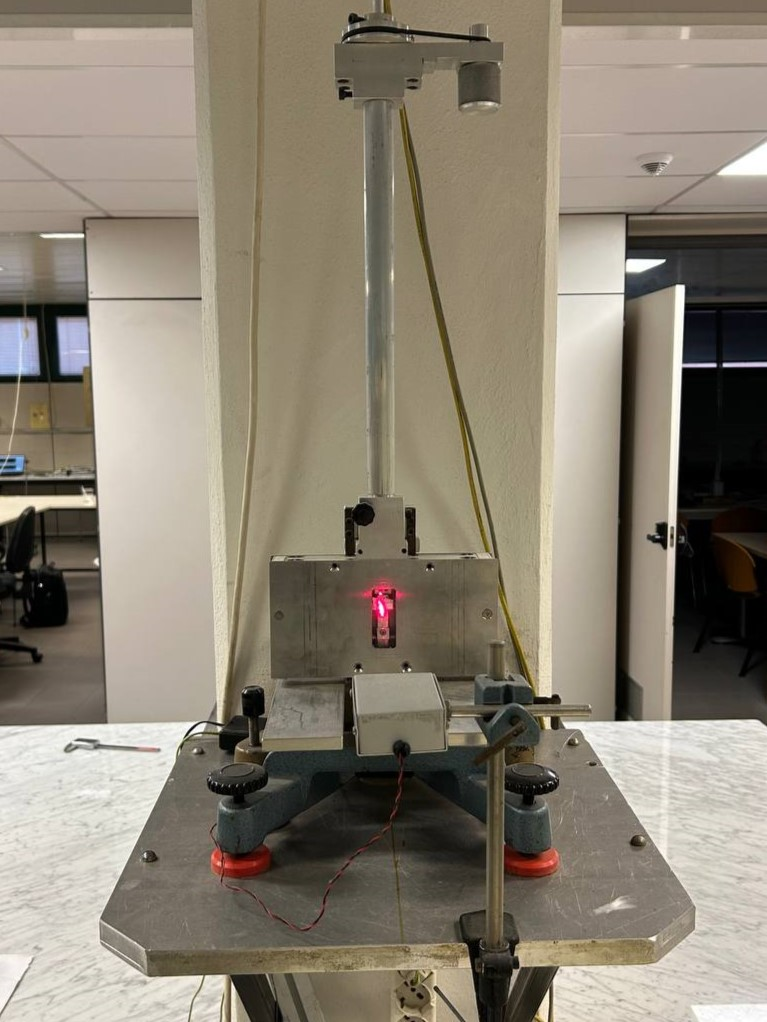
\includegraphics[width=0.3\linewidth]{images/setup.jpg}
    \caption{Il setup sperimentale visto dall'esterno. Le sferette sono contenute nella scatola metallica posta in basso, mentre il filo va dalla cima dell'apparato al centro del manubrio, che si trova nel punto in cui viene riflessa la luce rossa del laser.}
    \label{fig:setup}
\end{figure}

Le sferette, se sottoposte ad attrazione gravitazionale, iniziano ad oscillare attorno a una posizione d'equilibrio perché il filo risponde al momento della forza di gravità con un momento torcente pari in modulo e opposto in verso.
Per poter apprezzare sensibilmente il movimento dovuto all'interazione gravitazionale con le masse sorgenti, al centro del manubrio è posto uno specchio che riflette su uno schermo di carta millimetrata la luce di un laser (Fig. \ref{fig:laser}). L'oscillazione registrata è alla base dei calcoli che sono stati effettuati per ricavare la costante di gravitazione universale.

\begin{figure}[ht!]
    \centering
    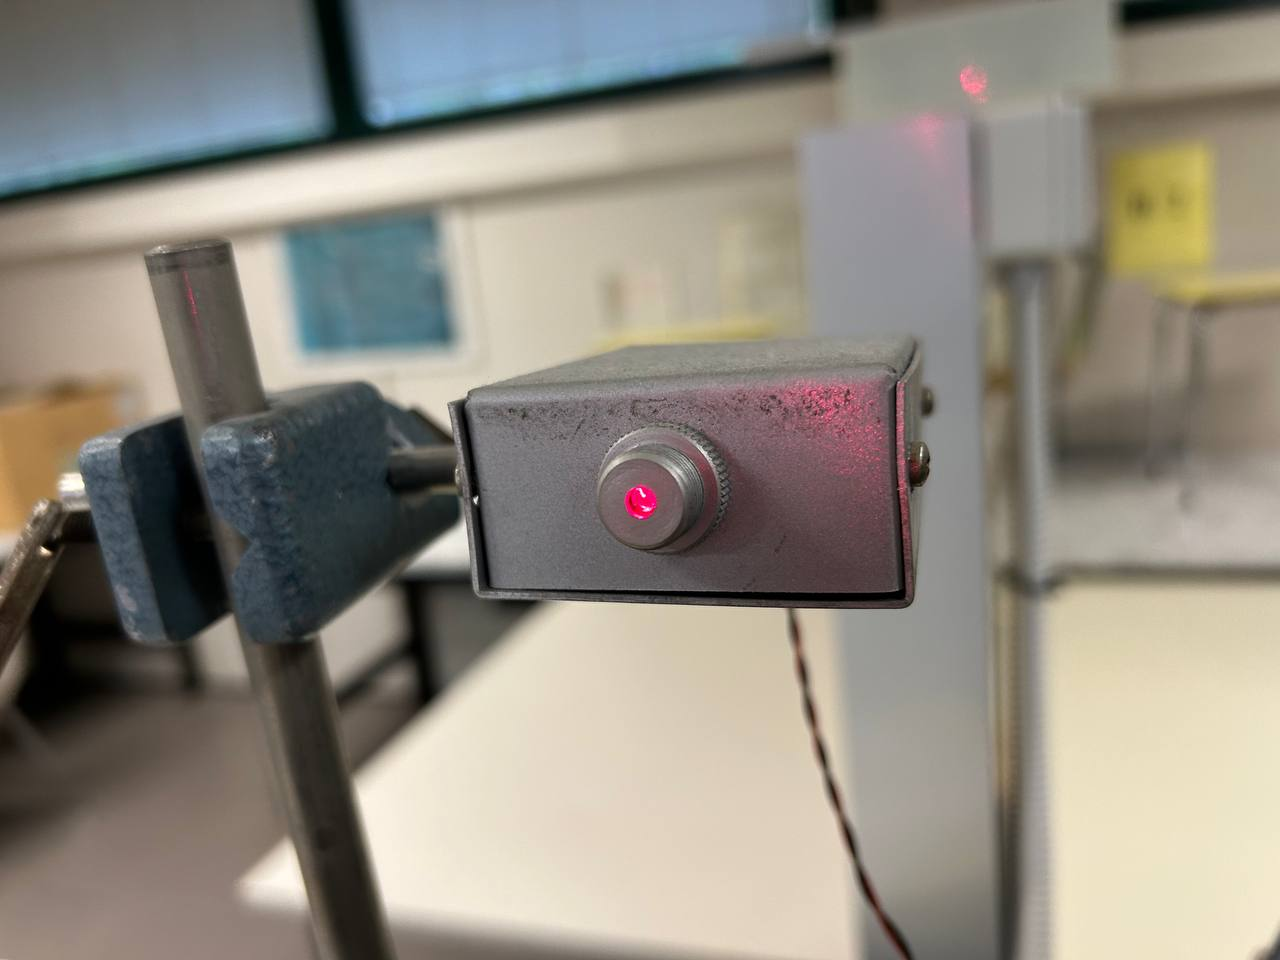
\includegraphics[width=0.3\linewidth]{images/laser.jpg}
    \hfill
    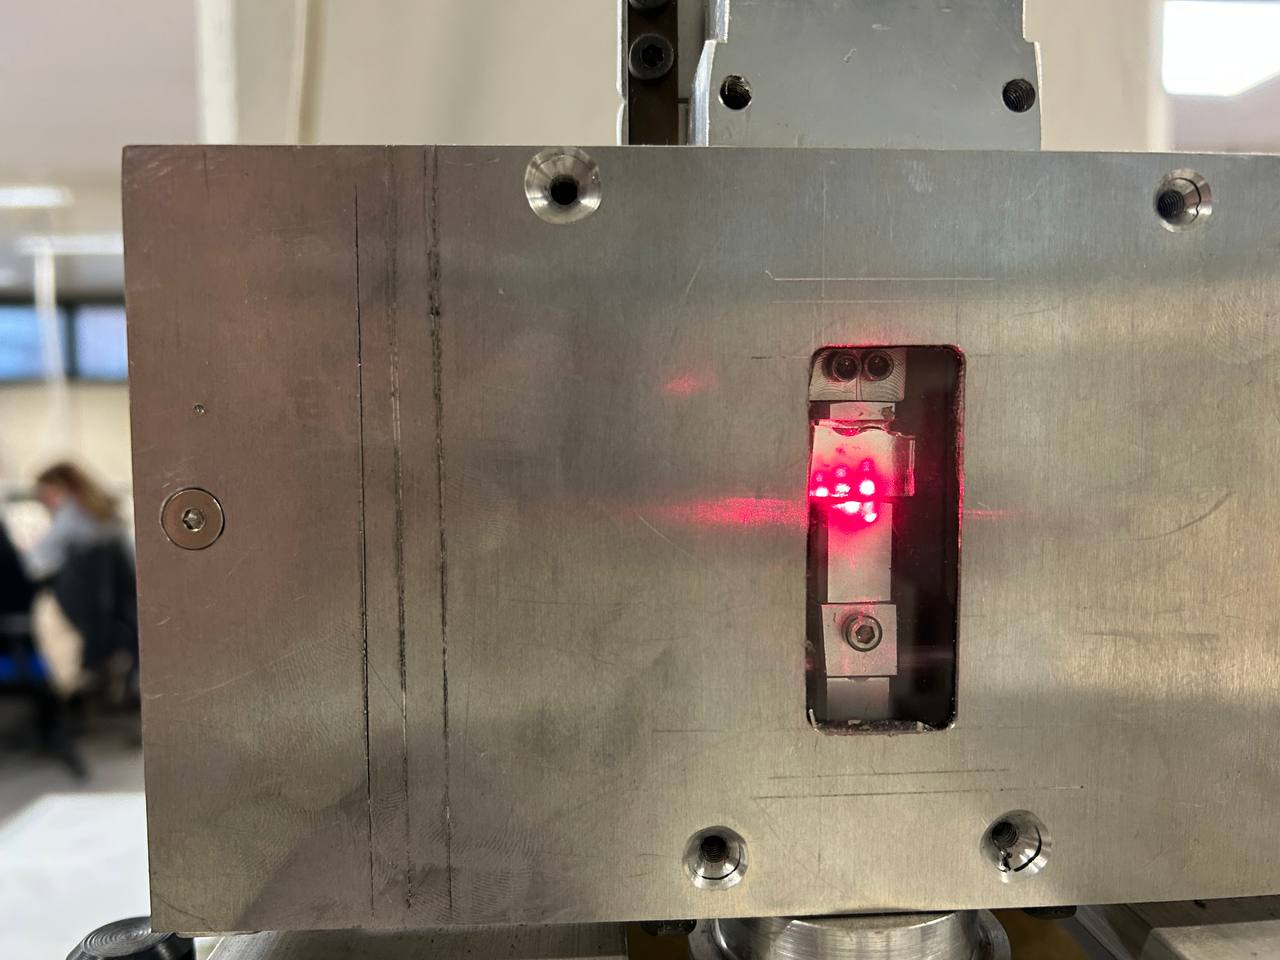
\includegraphics[width=0.3\linewidth]{images/mirror.jpg}
    \hfill
    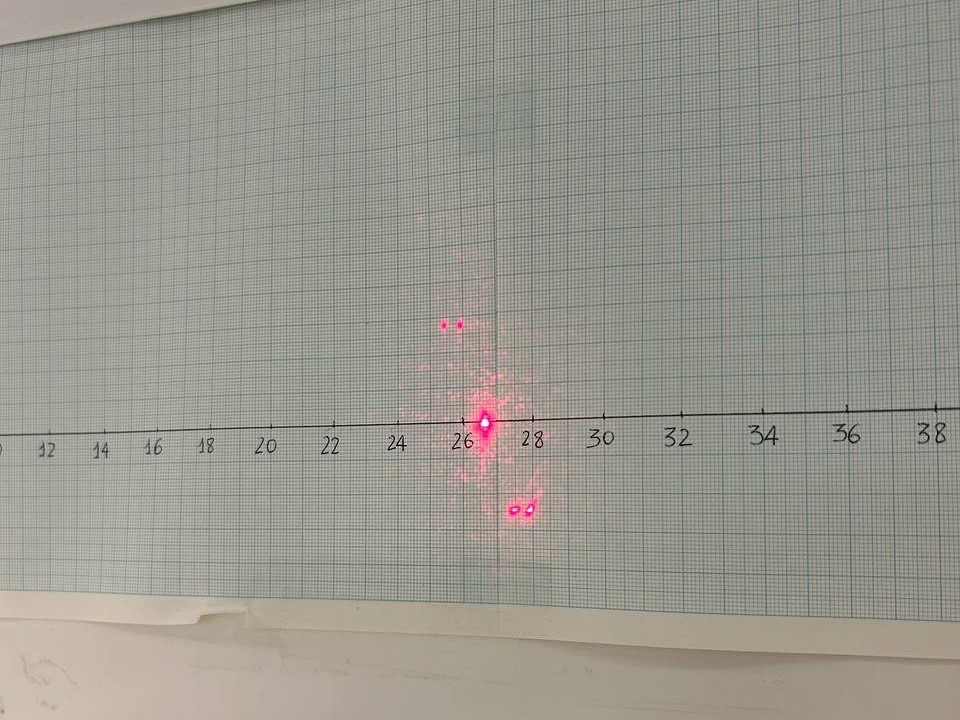
\includegraphics[width=0.3\linewidth]{images/monitor.jpg}
    \caption{Il laser viene prodotto dal macchinario nell'immagine a sinistra e, dopo essere stato riflesso dallo specchio montato sul manubrio (foto al centro), giunge su uno schermo di carta millimetrata (immagine a destra) per poterne apprezzare il movimento.}
    \label{fig:laser}
\end{figure}

\subsection{Svolgimento}
La raccolta dei dati è stata effettuata con due diverse configurazioni per poter calcolare il valore di $G$ tramite la seguente formula\footnote{Per la trattazione dettagliata si rimanda all'appendice.}:
\begin{equation}\label{eq:g}
    G = \frac{b ^ 2 \pi ^ 2 d (S_1 - S_2)}{M L T ^ 2} \left[1 + \frac{2}{5} \left(\frac{r}{d}\right) ^ 2\right]
\end{equation}
dove $b$ è la distanza tra il centro di una sferetta e l'asse del cilindro ad essa più vicino, $d$ è la distanza tra una sferetta e il centro del manubrio, $S_1$ e $S_2$ sono i punti in cui l'oscillazione del laser tende a stabilizzarsi nelle due differenti configurazioni, $M$ è la media delle masse dei cilindri, $L$ è la distanza tra lo schermo e lo specchietto, $T$ è il periodo delle oscillazioni del manubrio e $r$ è il raggio delle sferette. I valori di $d$ e $r$, essendo i componenti posti all'interno della scatola sigillata, erano noti a priori. Al contrario, $b$ è stato calcolato a partire dal lato della scatola metallica $l$ e dal diametro dei cilindri $D$ con la formula:

\begin{equation}\label{eq:b}
    b = \frac{1}{2} \left( l + D\right)
\end{equation}

Inizialmente sono state prese le misure relative alle masse sorgenti\footnote{Verranno trattate più in dettaglio nella sezione \ref{section:daq}.}, successivamente è stata effettuata la presa dati sulle due configurazioni e infine, per minimizzare il rischio di intaccare l'apparato sperimentale, sono state prese le misure geometriche del setup sperimentale. Per la prima configurazione, un cilindro è stato posto dietro la scatola sul supporto di destra (guardando lo schermo di carta millimetrata) e l'altro davanti alla scatola sul supporto di sinistra, in modo che fossero diametralmente opposti (Fig. \ref{fig:config_1}). La seconda configurazione, speculare alla prima, è stata realizzata spostando entrambi i cilindri dal lato opposto della scatola (Fig. \ref{fig:config_2}).\\
Con questo setup, per effetto della forza di attrazione gravitazionale si genera un momento torcente sul filo, il quale risponde con un momento torcente di richiamo che porta il filo a raggiungere una posizione di equilibrio, oscillando prima attorno ad essa. Ciascuna configurazione è stata analizzata per cinque oscillazioni complete, annotando ogni dieci secondi la posizione del laser sullo schermo di carta millimetrata.
$S_1$ e $S_2$ sono stati ricavati attraverso il pacchetto di analisi dati ROOT con un'apposita macro, ovvero un programma che ne sfrutta le funzionalità, per costruire un fit dell'oscillazione a partire dalle posizioni registrate durante la presa dati. Allo stesso modo è stato calcolato anche il periodo dell'oscillazione $T$, legato alla pulsazione $\omega$ ricavata dal fit dalla seguente relazione:
\begin{equation}\label{eq:periodo}
    T = \frac{2 \pi}{\omega}
\end{equation}

\begin{figure}[h!]
    \centering
    \begin{minipage}[t]{0.45\textwidth}
        \centering
        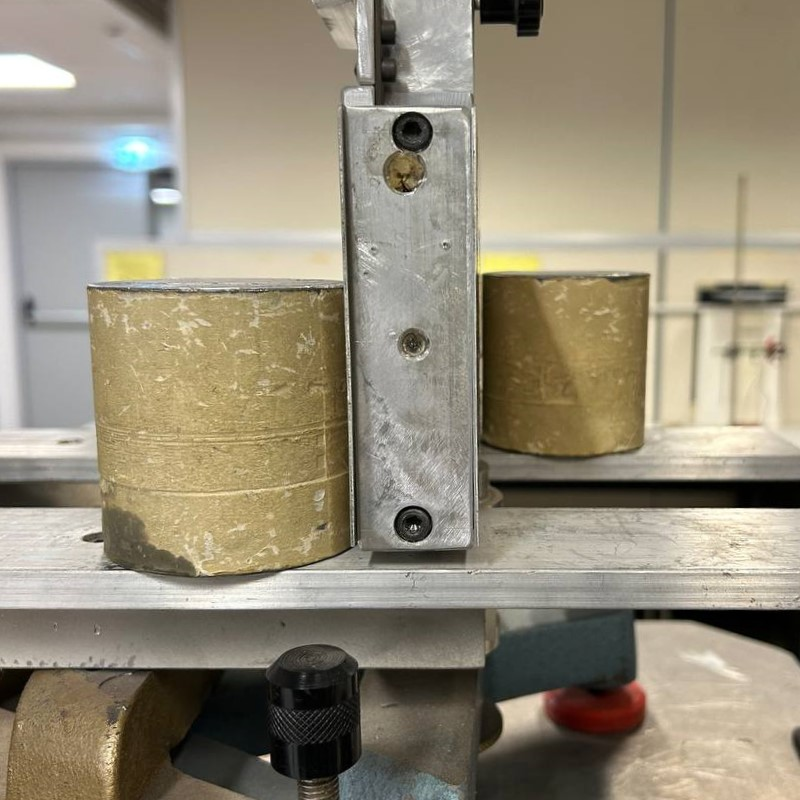
\includegraphics[width=\textwidth]{images/config_1.jpg}
        \caption{La prima configurazione, utilizzata per la misura di $S_1$. Al centro si trova la scatola contenente le sferette, affiancata dalle due masse sorgenti. Lo schermo millimetrato si trovava sulla destra da questo punto di vista.}
        \label{fig:config_1}
    \end{minipage}\hfill
    \begin{minipage}[t]{0.45\textwidth}
        \centering
        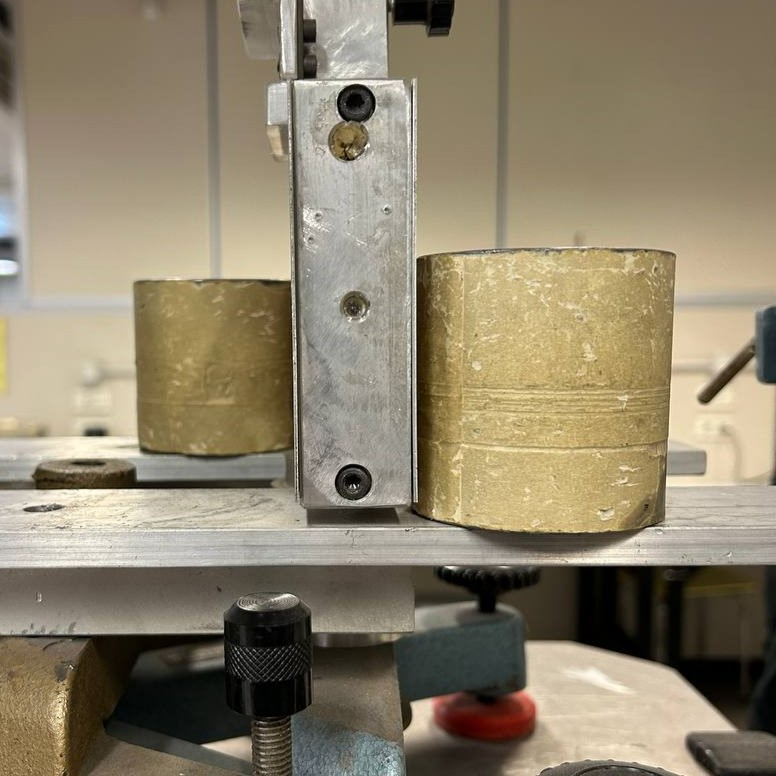
\includegraphics[width=\textwidth]{images/config_2.jpg}
        \caption{La seconda configurazione, utilizzata per la misura di $S_2$. È stata fotografata dalla stessa prospettiva della Fig. \ref{fig:config_1}, per cui anche in questo caso lo schermo millimetrato si trovava sulla destra.}
        \label{fig:config_2}
    \end{minipage}
\end{figure}

\section{Risultati}
\subsection{Acquisizione dati}\label{section:daq}
I valori della distanza tra le sferette e il centro del manubrio, $d$, e del raggio delle sferette, $r$, erano noti in partenza, poiché per misurarli si sarebbe dovuta aprire la scatola sigillata contenente le sferette. Inizialmente sono state misurate le caratteristiche delle masse sorgenti: la massa $M$ è la media delle masse $M_1$ e $M_2$, misurate con una bilancia (Fig. \ref{fig:bilancia}) di sensibilità $1 g$, a cui è stata associata come incertezza la semidispersione massima. Il diametro $D$ è stato calcolato come la media di sei misure, effettuate con un calibro (Fig. \ref{fig:calibro}) di sensibilità $0.01 mm$ su entrambi i cilindri. L'incertezza associata alla media delle sei misure corrisponde alla semidispersione massima del campione, ovvero $0.1 mm$. Dopo la presa dati è stato misurato il lato della scatola $l$ con lo stesso calibro utilizzato in precedenza. La distanza fra lo specchio e lo schermo, $L$, è stata misurata con un metro (Fig. \ref{fig:metro}) con sensibilità di $1 mm$. Il parametro $b$ è stato calcolato attraverso la formula (\ref{eq:b}) e la sua incertezza è stata ricavata propagando le incertezze\footnote{Per il calcolo delle incertezze si veda l'appendice.}. Nella tabella seguente (Tab. \ref{tab:daq}) sono riassunti i risultati della fase di misura.

\begin{table}[ht!]
    \centering
    \begin{tabular}{|c|c|c|}
    \hline
        Grandezza & Misura & Descrizione\\
        \hline
        $d$	&$(6.4225 \pm 0.0025)\times10^{-2} m$&Distanza sferetta-centro\\
        \hline
        $r$  &$(9.525 \pm 0.025)\times10^{-3}m$&Raggio sferette\\
        \hline
        $l$  &$(3.254 \pm 0.001)\times10^{-2} m$&Lato scatola\\
        \hline
        $D$ &$(6.77 \pm 0.01)\times10^{-2} m$&Diametro massa sorgente\\
        \hline
        $b$ &$(5.01 \pm 0.06)\times10^{-2} m$&Distanza sferetta-cilindro\\
        \hline
        $L$ &$(2.61 \pm 0.001) m$&Distanza schermo-specchio\\
        \hline
        $M_1$ &$(2.764 \pm 0.001) kg$&Massa cilindro 1\\
        \hline
        $M_2$ &$(2.750 \pm 0.001) kg$&Massa cilindro 2\\
        \hline
        $M$ & $(2.757 \pm 0.007) kg$ & Massa sorgente\\
        \hline
    \end{tabular}
    \caption{Nella tabella sono riportati i dati delle misure relative all'apparato sperimentale e alle masse sorgenti. Nella prima colonna è riportato il simbolo della grandezza presa in esame, nella seconda colonna il suo valore con la rispettiva incertezza e nella terza colonna la sua descrizione.}
    \label{tab:daq}
\end{table}

\begin{figure}[ht!]
    \centering
    \begin{minipage}[t]{0.3\linewidth}
        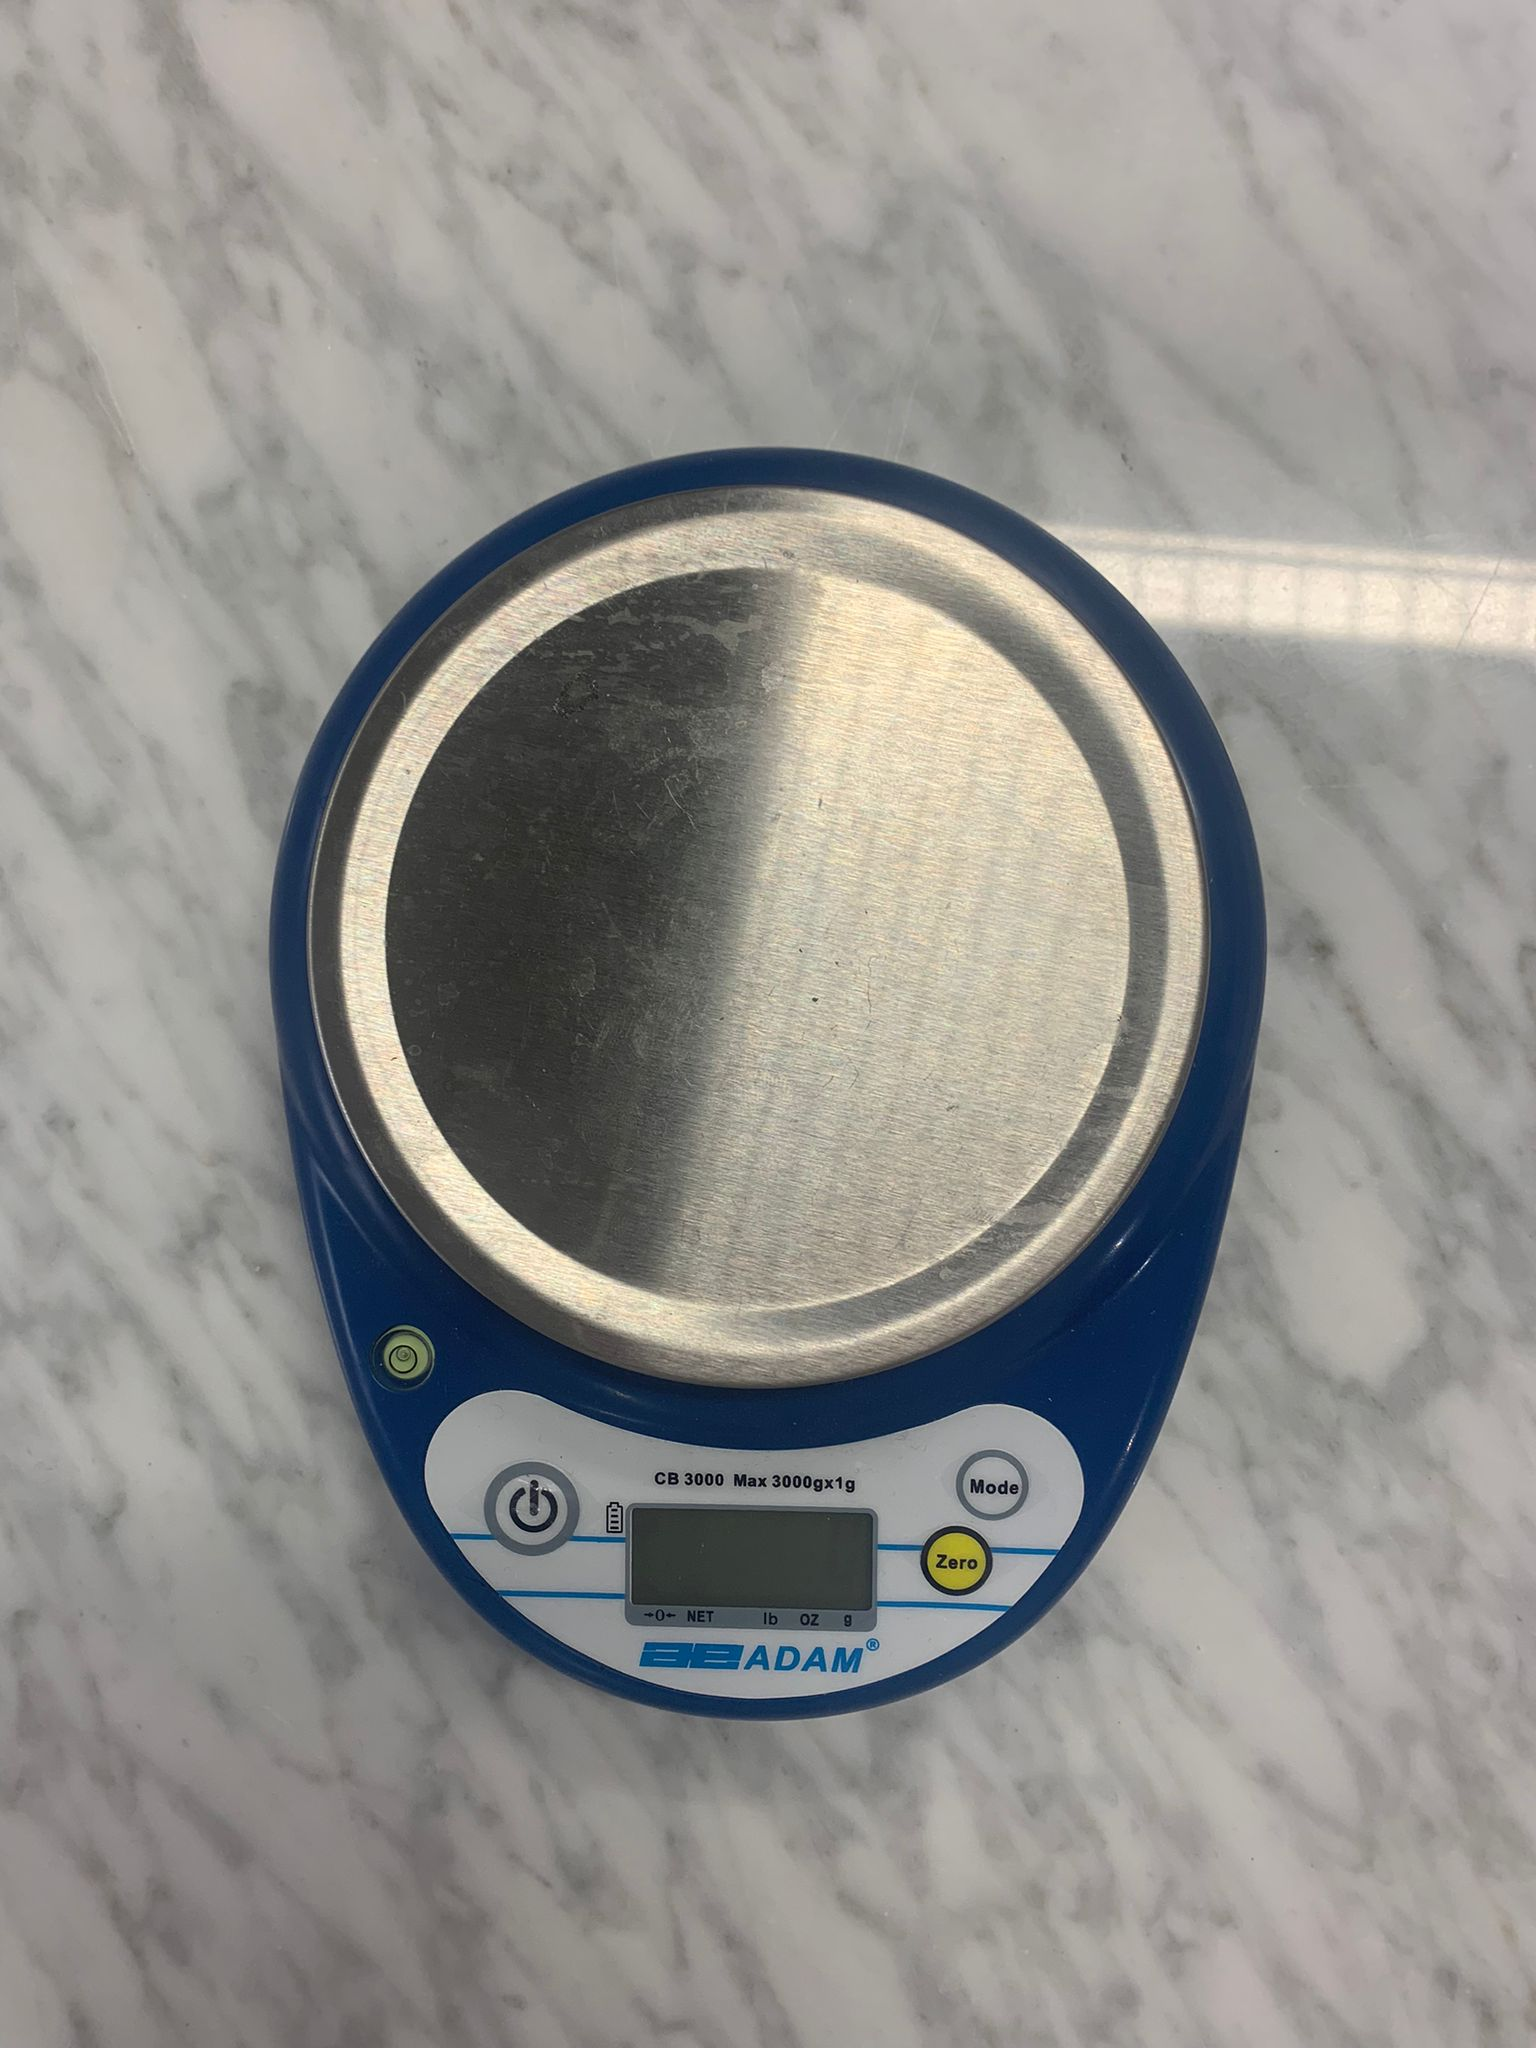
\includegraphics[width=\linewidth]{images/bilancia.jpeg}
        \caption{La bilancia utilizzata per misurare le masse sorgenti. Ha una sensibilità di $1g$.}
        \label{fig:bilancia}
    \end{minipage}\hfill
    \begin{minipage}[t]{0.3\linewidth}
        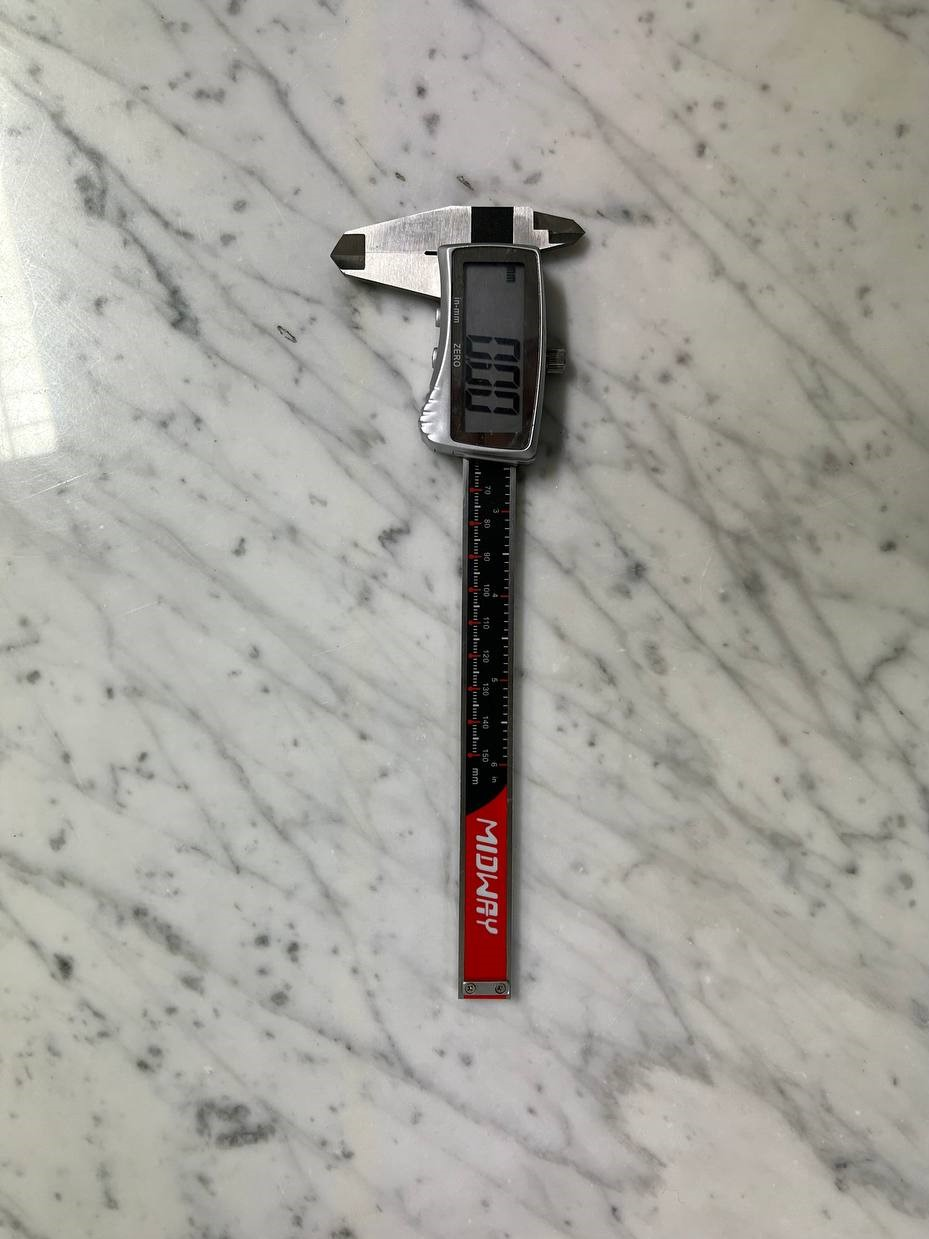
\includegraphics[width=\linewidth]{images/calibro.jpg}
        \caption{Il calibro di sensibilità $0.01mm$ utilizzato per le misure del diametro dei cilindri e del lato della scatola.}
        \label{fig:calibro}
    \end{minipage}\hfill
    \begin{minipage}[t]{0.3\linewidth}
        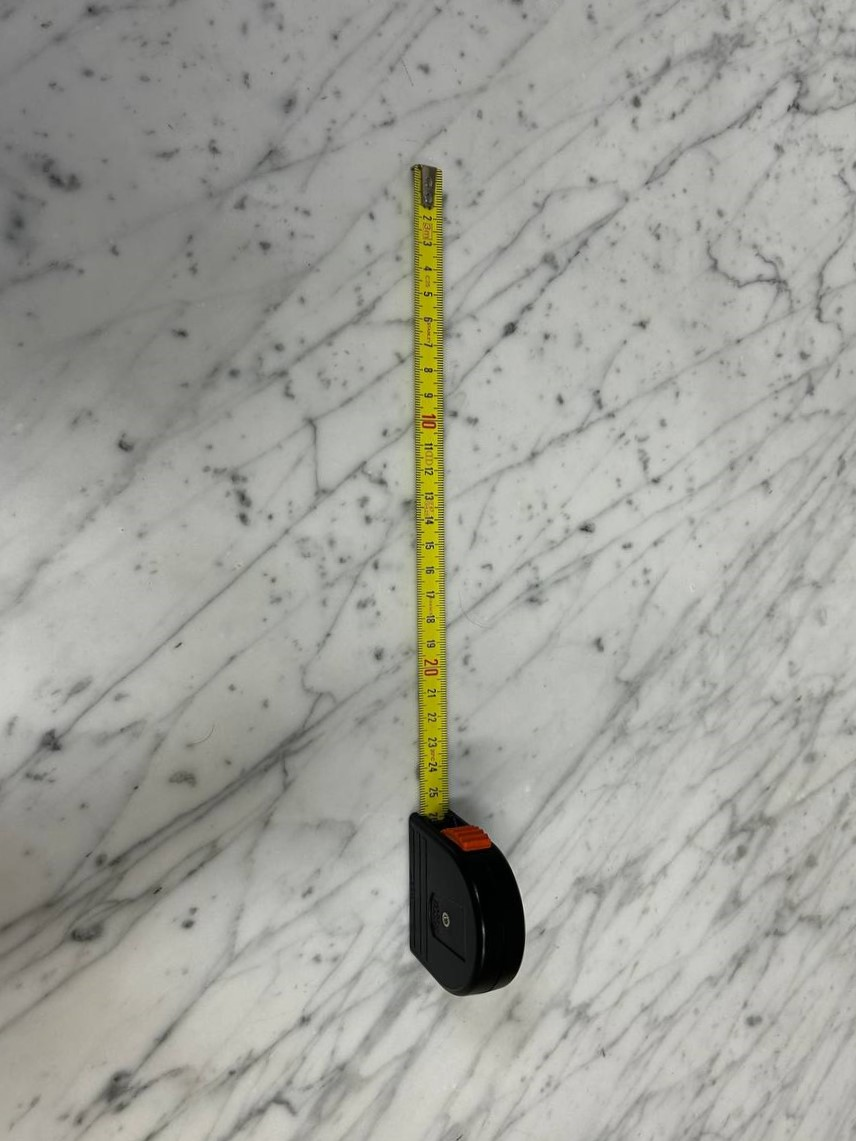
\includegraphics[width=\linewidth]{images/metro.jpg}
        \caption{Il metro utilizzato per misurare la distanza fra lo specchio e lo schermo. Ha una sensibilità di $1mm$.}
        \label{fig:metro}
    \end{minipage}
\end{figure}

I dati relativi alla posizione dello spot del laser durante le oscillazioni prese in esame sono stati annotati su un foglio di calcolo Excel osservando a intervalli di dieci secondi la posizione in cui il laser colpiva lo schermo di carta millimetrata. Successivamente, i dati raccolti sono stati analizzati e rappresentati graficamente con ROOT (Fig. \ref{fig:graph_1} e Fig. \ref{fig:graph_2}). Per ogni configurazione, tramite la macro, sono stati calcolati sei parametri (Tab. \ref{tab:parameters_1} e Tab. \ref{tab:parameters_2}) utili a realizzare un fit sui dati raccolti secondo la funzione che descrive un moto armonico smorzato:
\begin{equation}
    x(t)=p_0\sin(p_1t + p_2)\ e^{-\frac{t}{p_3}}\\ + p_4 +p_5t
\end{equation}

\begin{itemize}
    \item$p_0$ rappresenta l'ampiezza dell'oscillazione;
    \item$p_1$ rappresenta la pulsazione con cui sono avvenute le oscillazioni;
    \item $p_2$ rappresenta l'angolo di fase dell'oscillazione;
    \item$p_3$ rappresenta la costante di decadimento del moto armonico smorzato, ossia il tempo necessario affinchè l'ampiezza dell'oscillazione si riduca di un fattore pari a $e$;
    \item $p_4$ rappresenta l'ordinata all'origine della retta di deriva (dopo opportune correzioni corrisponde a $S_1$ o a $S_2$, a seconda della configurazione);
    \item $p_5$ rappresenta il coefficiente angolare della retta di deriva.
\end{itemize}
Tramite i parametri $p_4$ e $p_5$ è stata rappresentata la retta di deriva nei grafici a sinistra delle Figure \ref{fig:graph_1} e \ref{fig:graph_2}, che non risulta costante a causa di un \textit{kick} iniziale dovuto all'avvicinamento delle masse sorgenti che porta il manubrio a non oscillare immediatamente attorno alla posizione di equilibrio. Per minimizzare l'influenza di questo effetto sistematico sulla presa dati, sono state prese in esame cinque oscillazioni per ogni configurazione, lasciando quindi passare un intervallo di tempo sufficiente per far dissipare l'effetto del \textit{kick}. Il valore cercato della posizione di equilibrio risulta essere la posizione finale della retta di deriva, valore che indica il punto attorno cui avviene l'oscillazione solamente ad opera del momento torcente gravitazionale e del momento di richiamo. Per questo motivo, nei grafici a destra delle Figure \ref{fig:graph_1} e \ref{fig:graph_2} i parametri $p_4$ e $p_5$ sono stati corretti per rappresentare un'oscillazione attorno a un punto di equilibrio costante (rispettivamente $S_1$ e $S_2$).

Di seguito sono riportati i grafici (Fig. \ref{fig:graph_1}) ottenuti dalla macro di ROOT e una tabella riassuntiva (Tab. \ref{tab:parameters_1}) dei dati raccolti per la prima configurazione.

\begin{figure}[ht!]
    \centering
    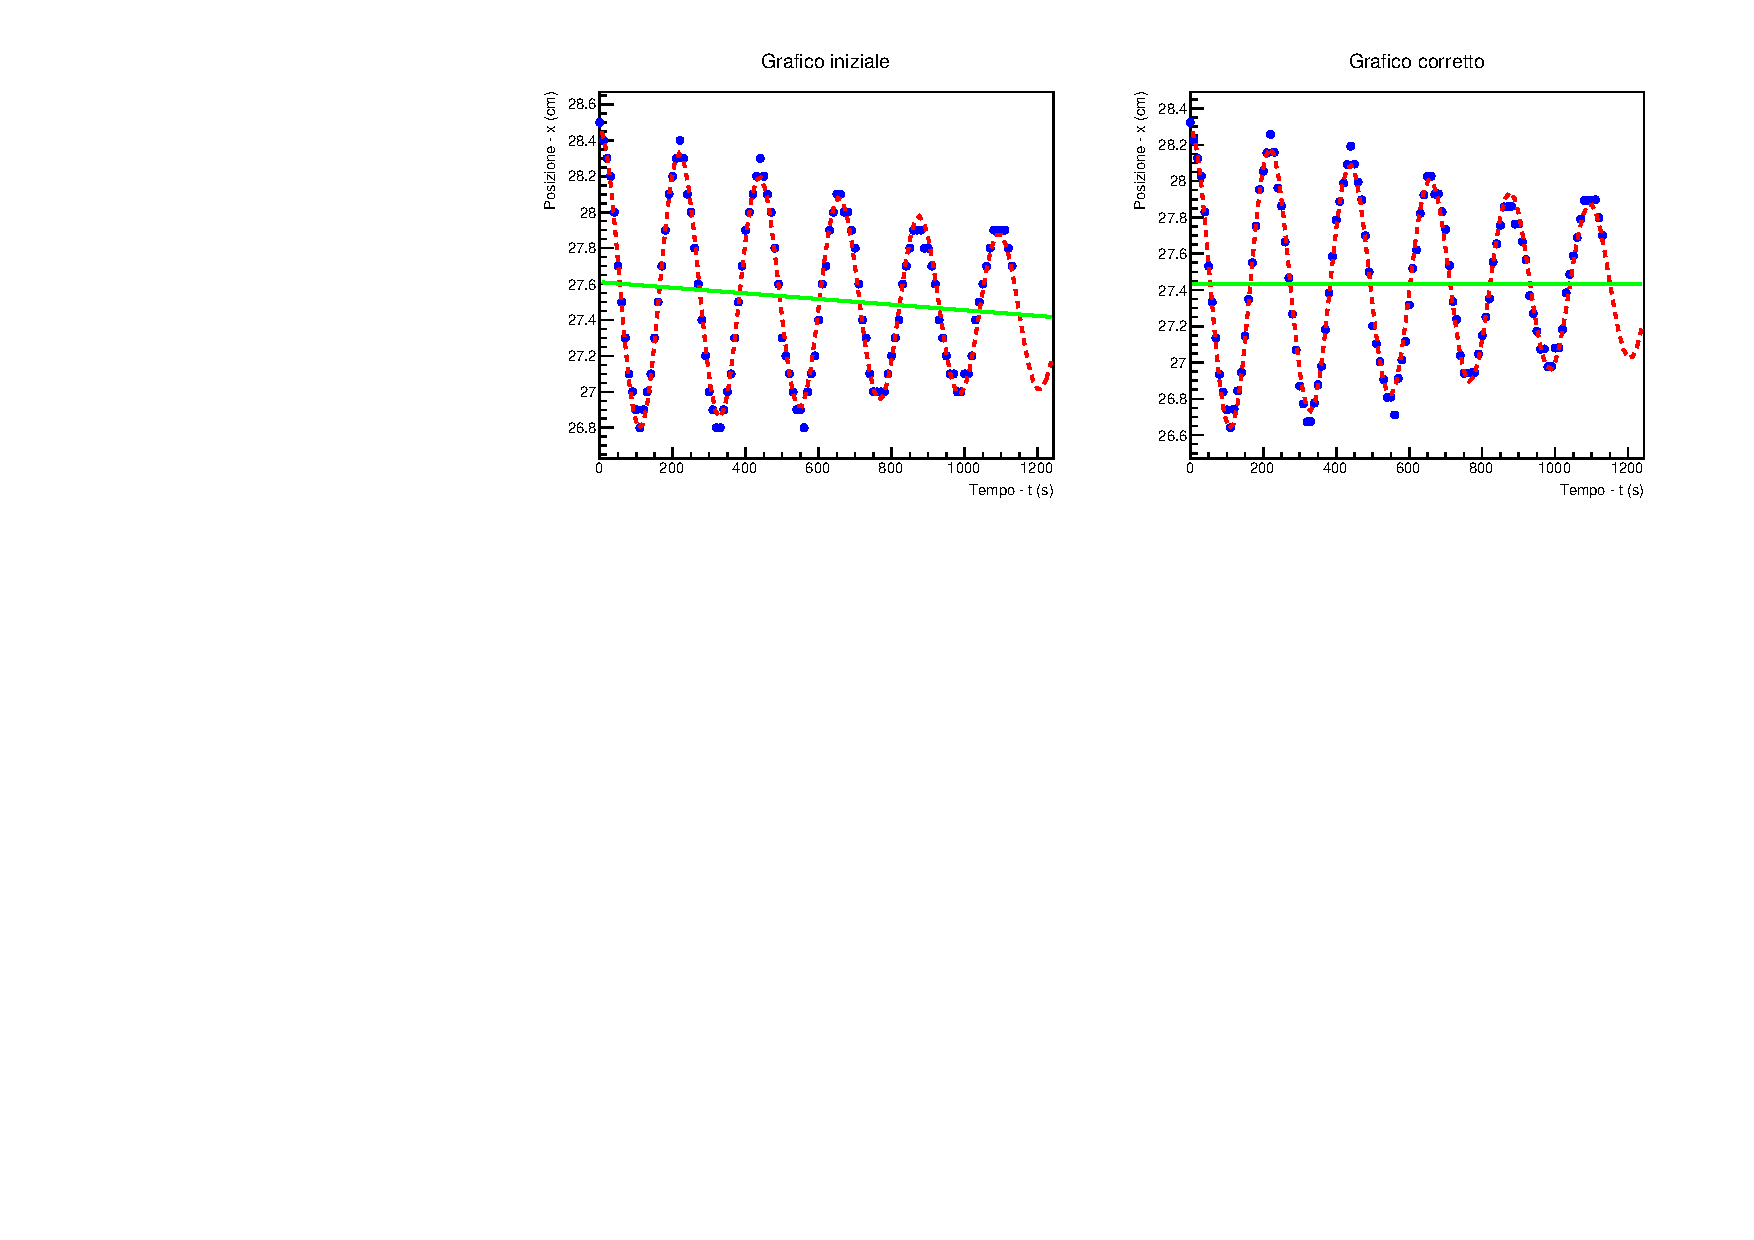
\includegraphics[width=1\linewidth]{images/graphS1.pdf}
    \caption{I due grafici rappresentano il movimento delle sferette nella prima configurazione. L'asse delle ascisse indica il tempo ($s$), l'asse delle ordinate indica la posizione del laser ($cm$). I punti blu rappresentano i dati raccolti della posizione dello spot del laser sullo schermo di carta millimetrata. La linea tratteggiata rossa rappresenta l'andamento sinusoidale dello spot attorno alla posizione di equilibrio. La linea continua verde rappresenta la deriva lineare della posizione di equilibrio. Nel grafico a sinistra si può notare il kick iniziale, mostrato da una retta di deriva con pendenza negativa. Il grafico a destra, tramite un'opportuna correzione, rappresenta come una retta costante la posizione di equilibrio $S_1$ attorno a cui oscilla lo spot del laser.}
    \label{fig:graph_1}
\end{figure}

\newpage

\begin{table}[ht!]
    \centering
    \begin{tabular}{|c|c|c|}
        \hline
        Simbolo & Grafico iniziale & Grafico corretto \\
        \hline
        $p_0$ & \multicolumn{2}{c|}{$(-8.55 \pm 0.16)\times10^{-3}m$}\\
        \hline
        $p_1$ & \multicolumn{2}{c|}{$(2.868 \pm 0.004)\times10^{-2}rad/s$}\\
        \hline
        $p_2$ & \multicolumn{2}{c|}{$(1.099 \pm 0.002)\times10rad$}\\
        \hline
        $p_3$ & \multicolumn{2}{c|}{$(1.65 \pm 0.09)\times10^{3}$s}\\
        \hline
        $p_4$ & $(2.7611 \pm 0.0010)\times10^{-1}m$& $(2.7434 \pm 0.0010)\times10^{-1}m$ \\
        \hline
        $p_5$ & $(-1.56 \pm 0.15)\times10^{-6}m/s$ & $(0 \pm 0.15)\times10^{-6}m/s$\\
        \hline
        \hline
        $T_1$ & \multicolumn{2}{c|}{$(219.1 \pm 0.3)s$}\\
        \hline
        $S_1$ & \multicolumn{2}{c|}{$(2.74 \pm 0.01)\times10^{-1}m$}\\
        \hline
    \end{tabular}
    \caption{La tabella mostra i valori dei parametri calcolati con ROOT a partire dai dati raccolti durante la prima configurazione. I parametri da $p_0$ a $p_3$ rimangono costanti per entrambi i grafici, mentre variano i parametri $p_4$ e $p_5$. Questi ultimi rappresentano rispettivamente l'ordinata all'origine e il coefficiente angolare della retta di deriva. Nel grafico di sinistra descrivono la retta di deriva calcolata dai dati, mentre nel grafico di destra, dopo un'opportuna correzione, si ha $p_5 \approx 0$ e $p_4$ che rappresenta la posizione di equilibrio $S_1$ con incertezza di $1mm$ dovuta alla risoluzione dello schermo di carta millimetrata. Il periodo $T_1$ e la sua incertezza sono stati calcolati a partire dal parametro $p_1$ tramite la relazione \eqref{eq:periodo}.}
    \label{tab:parameters_1}
\end{table}

È stato seguito lo stesso procedimento per la seconda configurazione, di cui sono riportati i grafici (Fig. \ref{fig:graph_2}) e la tabella (Tab. \ref{tab:parameters_2}) con tutti i parametri, il periodo d'oscillazione e la posizione d'equilibrio.
 
\begin{figure}[ht!]
    \centering
    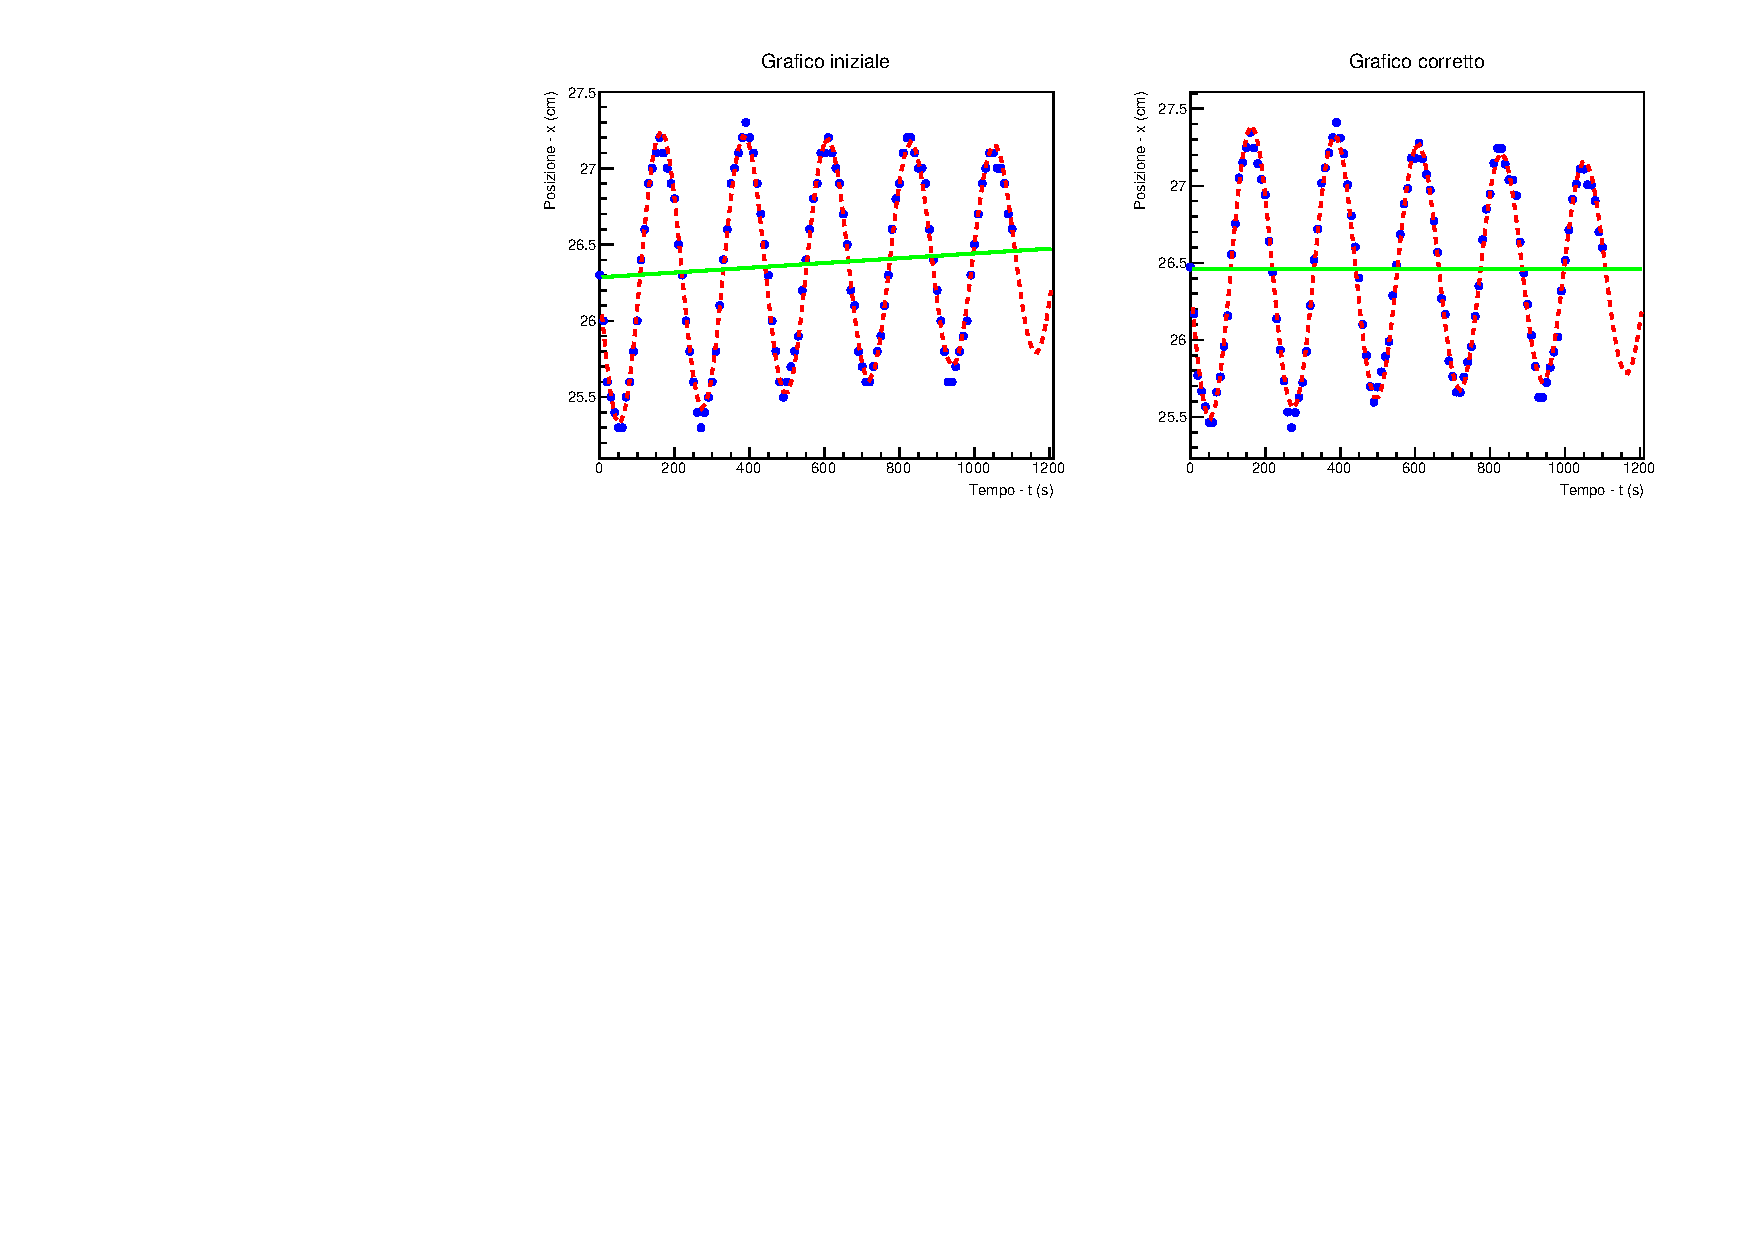
\includegraphics[width=1\linewidth]{images/graphS2.pdf}
    \caption{I grafici rappresentano l'oscillazione delle sferette con la seconda configurazione. L'asse delle ascisse indica il tempo ($s$), l'asse delle ordinate indica la posizione del laser ($cm$). In entrambi i grafici i punti blu rappresentano la posizione dello spot del laser. La sinusoide tratteggiata di colore rosso è calcolata tramite la macro di ROOT, che a partire dai dati raccolti della posizione dello spot realizza un fit sinusoidale dell'oscillazione attorno alla posizione di equilibrio. Il grafico a sinistra mostra il kick iniziale imposto dal posizionamento delle masse sorgenti. Ne risulta una retta di deriva con pendenza positiva, colorata in verde. Nel grafico di destra, sottraendo la deriva tramite la macro di ROOT, la retta verde continua risulta costante. Il valore di questa retta rappresenta la posizione di equilibrio $S_2$ attorno cui oscilla lo spot del laser e coincide col valore di $p_4$.}
    \label{fig:graph_2}
\end{figure}

\newpage

\begin{table}[ht!]
     \centering
     \begin{tabular}{|c|c|c|}
         \hline
         Simbolo & Grafico iniziale & Grafico corretto \\
         \hline
         $p_0$ & \multicolumn{2}{c|}{$(-9.8 \pm 0.2)\times10^{-3}m$} \\
         \hline
         $p_1$ & \multicolumn{2}{c|}{$(2.828 \pm 0.003)\times10^{-2}rad/s$} \\
         \hline
         $p_2$ & \multicolumn{2}{c|}{$(8.4 \pm 1.9)\times10^{-2}rad$} \\
         \hline
         $p_3$ & \multicolumn{2}{c|}{$(3.2 \pm 0.3)\times10^{3}s$} \\
         \hline
         $p_4$ & $(2.6286 \pm 0.0013)\times10^{-1}m$ & $(2.6458\pm 0.0013)\times10^{-1}m$ \\
         \hline
         $p_5$ & $(1.6 \pm 0.2)\times10^{-6}m/s$ & $(0 \pm 0.2)\times10^{-6}m/s$ \\
         \hline
         \hline
         $T_2$ & \multicolumn{2}{c|}{$(222.2 \pm 0.2)s$} \\
         \hline
         $S_2$ & \multicolumn{2}{c|}{$(2.65\pm 0.01)\times10^{-1}m$} \\
         \hline
     \end{tabular}
     \caption{Con la macro di ROOT sono stati analizzati i dati raccolti con la seconda configurazione per calcolare i parametri inseriti in tabella. Si può notare che, come nel caso della prima configurazione, i parametri da $p_0$ a $p_3$ rimangono costanti fra i due grafici. Al contrario, $p_4$ e $p_5$ sono stati modificati tramite la macro per mostrare una retta costante ($p_5 \approx 0$) sulla posizione di equilibrio ($p_4 \equiv S_2$), anche in questo caso con incertezza di $1mm$ per via della risoluzione dello schermo di carta millimetrata. Il periodo $T_2$ e la sua incertezza sono stati calcolati grazie al parametro $p_1$ tramite la relazione \eqref{eq:periodo}.}
     \label{tab:parameters_2}
\end{table}

\subsection{Elaborazione dati e risultati quantitativi}
Il valore di $G$ è stato calcolato tramite la formula \eqref{eq:g} con i dati raccolti in precedenza. Il periodo $T$ è stato calcolato come la media dei periodi $T_1$ e $T_2$, con incertezza corrispondente alla semidispersione massima fra le due misure. L'incertezza sulla grandezza $(S_1 - S_2)$ è stata calcolata sommando i valori assoluti delle incertezze associate alle misure di $S_1$ e $S_2$.
È stato possibile ricavare l'incertezza relativa associata alla misura di $G$ tramite la formula seguente\footnote{Per la derivazione della formula si rimanda all'appendice.}:
\begin{equation}\label{eq:epsilon}
    \epsilon_G = \frac{\Delta G}{G} = 2 \frac{\Delta b}{b} + 2 \frac{\Delta T}{T} + \frac{\Delta d}{d} + \frac{\Delta \left( S_1 - S_2 \right)}{S_1 - S_2} + \frac{\Delta M}{M} + \frac{\Delta L}{L}
\end{equation}
Conoscendo il valore di $G$ è stato dunque possibile calcolare $\Delta G = G \cdot \epsilon_G$. Nella tabella seguente (Tab. \ref{tab:incertezze_relative}) sono riportati i contributi a $\Delta G$ di ciascun parametro necessario al calcolo di $G$.
\begin{table}[ht!]
    \centering
    \begin{tabular}{|c|c|c|c|c|c||c|}
        \hline
        $2 \frac{\Delta b}{b}$ & $2 \frac{\Delta T}{T}$ & $\frac{\Delta d}{d}$ & $\frac{\Delta \left(S_1 - S_2 \right)}{S_1 - S_2}$ & $\frac{\Delta M}{M}$ & $\frac{\Delta L}{L}$ & $\epsilon_G = \frac{\Delta G}{G}$ \\
        \hline
        $0.22\%$ & $1.41\%$ & $0.04\%$ & $20.49\%$ & $0.25\%$ & $0.04\%$ & $22.45\%$\\
        \hline
    \end{tabular}
    \caption{In tabella sono riportate le incertezze relative di ciascun parametro che compare nella formula per calcolare $G$. Si noti che la grandezza che contribuisce maggiormente ad aumentare il valore di $\epsilon_G$ è $S_1 - S_2$.}
    \label{tab:incertezze_relative}
\end{table}

Il valore di $G$ così misurato, $\displaystyle G=(4.5 \pm 1.0)\times10^{-11}\frac{Nm^{2}}{kg^{2}}$, necessita di una correzione per due effetti sistematici. Innanzitutto, le sferette all'interno della scatola risentono dell'attrazione gravitazionale di entrambe le masse sorgenti. Questo fatto non è stato tenuto in conto nel modello adottato per i calcoli, in cui è stata considerata solo la forza gravitazionale esercitata da ciascuna massa sorgente sulla sferetta a essa più prossima. Su entrambe le sferette agisce quindi un'altra forza, che contribuisce a frenare la rotazione del manubrio. Per tenere conto di quest'ultima è necessario introdurre il parametro $\beta$, calcolato mediante la formula:
\begin{equation}\label{eq:beta}
    \beta = \frac{b^{3}}{(b^{2}+4d^{2})^{3/2}}
\end{equation}
Il secondo effetto sistematico è causato dalla forma cilindrica delle masse sorgenti. Le formule utilizzate nei calcoli sono valide quando sia le masse sorgenti sia le masse di prova sono sferiche, quindi considerabili come puntiformi per il teorema dei gusci sferici\cite{focardi}. Per correggere l'effetto sistematico, il valore ottenuto di $G$ è stato moltiplicato per un fattore correttivo $f_c=1.1148$.
Sono stati applicati entrambi i fattori di correzione al valore misurato della costante $G$ secondo la formula:

\begin{equation}
    G_{corretto}=f_c\frac{G_{misurato}}{1-\beta}
\end{equation}
Tenendo conto dei fattori di correzione è stata calcolata nuovamente l'incertezza su $G$, che risulta essere\footnote{Per i calcoli estesi si rimanda all'appendice.}:
\begin{equation}
    \Delta G_{corretto} = \frac{f_c}{1 - \beta} \left( \Delta G_{misurato} + \frac{G_{misurato}}{1 - \beta} \Delta \beta \right)
\end{equation}
Il valore di $G$ dopo le correzioni corrisponde a $\displaystyle G=(5.2 \pm 1.2)\times10^{-11}\frac{Nm^{2}}{kg^{2}}$.

\section{Conclusioni}
Il valore di $G$ calcolato inizialmente è $\displaystyle G=(4.5 \pm 1.0)\times10^{-11}\frac{Nm^{2}}{kg^{2}}$, che non è compatibile con il valore atteso $\displaystyle G = (6.67430 \pm 0.00015)\times10^{-11}\frac{Nm^{2}}{kg^{2}}$, in quanto vi è una discrepanza significativa fra i due valori. Applicando i fattori di correzione si ottiene un ulteriore risultato di $\displaystyle G=(5.2 \pm 1.2)\times10^{-11}\frac{Nm^{2}}{kg^{2}}$.
Anche questo risultato non è compatibile con il valore accettato della costante di gravitazione universale, poiché anche in questo caso tra i due sussiste una discrepanza significativa.

\newpage

\section*{Appendice}
\paragraph{Calcolo di $G$}
Considerando l'angolo di deflessione molto piccolo, i bracci $\vec{r_1}$ e $\vec{r_2}$ possono essere approssimati con la distanza delle sferette dal centro, $\vec{d}$.
\begin{center}
\begin{tikzpicture}[baseline=(current bounding box.north)]
    \node[anchor=north, font=\bfseries\large] at (1.5,2) {Stato iniziale};
    % Sferette
    \shade[ball color=black] (0,0) circle (0.1);
    \shade[ball color=black] (3,0) circle (0.1);
    % Segnetto sul centro del segmento
    \draw (1.5,-0.1) -- (1.5,0.1);
    % Vettore d verso sinistra
    \draw[->] (1.5,0) -- (0.1,0) node[midway, above] {$\vec{d_1}$};
    % Vettore d verso destra
    \draw[->] (1.5,0) -- (2.9,0) node[midway, above] {$\vec{d_2}$};
\end{tikzpicture}
\hspace{2cm}
\begin{tikzpicture}[baseline=(current bounding box.north)]
    \node[anchor=north, font=\bfseries\large] at (1.5,2) {Stato finale};
    % Sferette
    \shade[ball color=black] (0,0.1) circle (0.1);
    \shade[ball color=black] (3,-0.1) circle (0.1);
    % Masse sorgenti
    \shade[ball color=white] (0,0.7) circle (0.5);
    \shade[ball color=white] (3,-0.7) circle (0.5);
    % Distanza b
    \draw[<->] (-0.6,0.7) -- (-0.6,0.1) node[midway, left] {$b$};
    \draw[<->] (3.6,-0.7) -- (3.6,-0.1) node[midway, right] {$b$};
    % Segnetto sul centro del segmento
    \draw (1.5,-0.1) -- (1.5,0.1);
    % Linea tratteggiata per la posizione iniziale
    \draw[dashed] (0,0) -- (3,0);
    % r1
    \draw[->] (1.5, 0) -- (0.1,0.1) node[midway, above] {$\vec{r_1}$};
    % r2
    \draw[->] (1.5, 0) -- (2.9,-0.1) node[midway, below] {$\vec{r_2}$};
\end{tikzpicture}
\end{center}
Di conseguenza,
\begin{align}
    \vec{M_g}
    &= \vec{r_1} \times \vec{F_1} + \vec{r_2} \times \vec{F_2} =\notag\\
    &= (-d\hat{i})\times(-F_1\hat{j}) + (d\hat{i})\times(F_2\hat{j}) =\notag\\
    &= dF_1\hat{k} + dF_2\hat{k} = 2dF\hat{k}\label{eq:torque}
\end{align}
Nell'equazione \eqref{eq:torque} $F$ è $\displaystyle F=G\frac{mM}{b^2}$, dove $m$ è la massa delle sferette e $M$ è la massa delle masse sorgenti, di conseguenza:
\begin{equation}\label{eq:Mg}
    \vec{M_g} = 2dG\frac{mM}{b^2}\hat{k}
\end{equation}

Come accennato nella sezione \ref{section:setup}, il filo risponde alla sollecitazione con un momento torcente uguale in modulo e contrario in verso a quello della forza gravitazionale. Il momento torcente è direttamente proporzionale a $\theta$, la deformazione angolare, e $K$, il modulo di torsione specifico del filo.
\begin{equation}\label{eq:Mr}
    \vec{M_r} = -K\theta\hat{k}
\end{equation}
Sommando la \eqref{eq:Mg} e la \eqref{eq:Mr} e ponendo la loro somma uguale a 0, si giunge alla seguente uguaglianza:
\begin{equation}
    2dG\frac{mM}{b^2}=K\theta
\end{equation}
Il modulo di torsione \cite{focardi} si può ricavare dinamicamente conoscendo la relazione che lo lega alla velocità angolare e quindi al periodo dell'oscillazione del laser attorno alle due posizioni di equilibrio $S_1$ e $S_2$.
\begin{equation}
    \omega ^ 2 = \left(\frac{2\pi}{T}\right)^2 = \frac{K}{I}
\end{equation}
Il momento d'inerzia $I$ è il doppio di quello di una sfera di raggio $r$ che ruota attorno a un asse parallelo a quello passante per il suo centro di massa. Per il teorema di Huygens-Steiner\cite{focardi},
\begin{equation}
    I = 2\left[\frac{2}{5}mr^2 + md^2\right] = 2md^2\left[1 + \frac{2}{5}\left(\frac{r}{d}\right) ^ 2 \right]
\end{equation}

\newpage

\begin{figure}
    \begin{minipage}{0.48\textwidth}
        \centering
        \begin{tikzpicture}
            % Segmento verso S_2
            \draw (0,0) -- (4,3);
            \node at (4.3,3) {$S_2$};
            % Segmento verso S_1
            \draw (0,0) -- (4,-3);
            \node at (4.3,-3) {$S_1$};
            % Bisettrice dell'angolo 2theta
            \draw[dotted, rotate={atan(3/4)/2}] (0,0) -- (3,0);
            % Schermo
            \draw (4,-3.5) -- (4,3.5);
            % Retta L
            \draw (0,0) -- (4,0) node[pos=0.8, above] {L};
            % Angolo di 4theta
            \draw (4/5,-3/5) arc (-{atan(3/4)}:{atan(3/4)}:1cm);
            % Etichette per gli angoli di 2theta
            \node at (1.2,0.4) {$2\theta$};
            \node at (1.2,-0.4) {$2\theta$};
            % Specchio e manubrio finali
            \fill[black, rotate={atan(3/4)/2}] (-0.25,-0.25) rectangle (0,0.25);
            \draw[rotate={atan(3/4)/2}] (-0.25,-0.9) -- (-0.25,0.9);
            \fill[black, rotate={atan(3/4)/2}] (-0.25,-1) circle (0.1);
            \fill[black, rotate={atan(3/4)/2}] (-0.25,+1) circle (0.1);
        \end{tikzpicture}
    \end{minipage}
    \hfill
    \begin{minipage}{0.48\textwidth}
        Per misurare l'angolo $\theta$ si ricorre alle posizioni di equilibrio calcolate con ROOT, $S_1$ e $S_2$. Poichè l'angolo incidente è uguale all'angolo riflesso, il laser viene riflesso sullo schermo a un angolo $2\theta$ nelle posizioni $S_1$ e $S_2$, che sono simmetriche rispetto alla posizione iniziale del laser. Per questo motivo, indicando con $L$ la distanza dallo specchio allo schermo millimetrato, si ha che
        \begin{equation}\label{eq:theta_1}
            \frac{S_1-S_2}{L}=2\tan(2\theta)
        \end{equation}
        
        Approssimando $\tan(2\theta) \approx 2\theta$ per angoli molto piccoli, l'equazione \eqref{eq:theta_1} restituisce la seguente relazione:
        \begin{equation}
            \theta = \frac{S_1-S_2}{4L}
        \end{equation}
    \end{minipage}
\end{figure}

Unendo tutte le formule ricavate fino ad ora, si può concludere che:

\begin{align}
    2dG\frac{mM}{b^2} &= \left(\frac{2\pi}{T}\right)^2I\frac{S_1-S_2}{4L}\notag\\
    2dG\frac{mM}{b^2} &= \frac{\pi ^2}{T^2} 2md^2\left[1+\frac{2}{5}\left(\frac{r}{d}\right)^2\right] \frac{S_1-S_2}{L}\notag\\
    G\frac{M}{b^2} &= \frac{\pi^2}{T^2}d\left[1+\frac{2}{5}\left(\frac{r}{d}\right)^2\right]\frac{S_1-S_2}{L}\notag\\
    G &= \frac{b^2\pi^2d(S_1-S_2)}{MLT^2}\left[1+\frac{2}{5}\left(\frac{r}{d}\right)^2\right]
\end{align}

\paragraph{Calcolo di $\Delta b$}
Le incertezze su $l$ e $D$ sono incertezze massime, quindi è possibile stimare dall'alto l'incertezza su $b$ tramite una combinazione lineare dei moduli delle derivate parziali di $a$\cite{taylor}. In generale, se la grandezza $a = f(x_0, x_1, ..., x_n)$ è funzione di $x_0, x_1, ..., x_n$, allora l'incertezza su $a$ può essere maggiorata come segue:
\begin{equation}
    \Delta a \leqslant \sum_{j = 0}^n \abs{\frac{\partial a}{\partial x_j}} \Delta x_j
\end{equation}
Sapendo che $\displaystyle b = \frac{1}{2} \left( l + D \right)$, è possibile stimare $\Delta b$:
\begin{equation}
    \Delta b \leqslant \abs{\frac{\partial b}{\partial l}} \Delta l + \abs{\frac{\partial b}{\partial D}} \Delta D = \frac{1}{2} (\Delta l + \Delta D)
\end{equation}

\paragraph{Calcolo di $\Delta G$}
Per semplificare i calcoli è lecito operare un'approssimazione.
Dal calcolo di $G$ si sa che $\displaystyle \frac{2}{5} \left( \frac{r}{d} \right) ^ 2 \approx 8.9 \times 10 ^ {-3} \ll 1$, di conseguenza risulta che:
\begin{equation}
    G \approx \frac{b^2 \pi^2 d \left( S_1 - S_2 \right)}{M L T^2}
\end{equation}
Ora per calcolare $\Delta G$ si può utilizzare la formula per la propagazione delle incertezze in un monomio\cite{taylor}. In generale, se la grandezza $\displaystyle a = c \prod_{j = 0}^n x_j^{\alpha_j}$ (ove $c$ è una costante) si esprime come monomio delle grandezze $x_0, x_1, ..., x_n$, allora è possibile calcolare l'incertezza relativa su $a$ mediante la seguente formula:
\begin{equation}\label{eq:incertezza_monomio}
    \frac{\Delta a}{a} = \sum_{j = 0}^n \alpha_j \frac{\Delta x_j}{x_j}
\end{equation}
Applicando la \eqref{eq:incertezza_monomio} a $G$ segue che:

\begin{equation}
    \epsilon_G = \frac{\Delta G}{G} = 2 \frac{\Delta b}{b} + 2 \frac{\Delta T}{T} + \frac{\Delta d}{d} + \frac{\Delta \left( S_1 - S_2 \right)}{S_1 - S_2} + \frac{\Delta M}{M} + \frac{\Delta L}{L}
\end{equation}

\paragraph{Calcolo di $\Delta \beta$}
Analogamente a $b$, $\beta$ dipende da grandezze con incertezze massime, di conseguenza anche in questo caso bisogna utilizzare la somma lineare\cite{taylor}.\\
Si sa che $\displaystyle \beta = \frac{b ^ 3}{\left( b ^ 2 + 4 d ^ 2 \right) ^ {3 / 2}}$, dunque è possibile stimare $\Delta \beta$:
\begin{align}
    \Delta \beta &\leqslant \abs{\frac{\partial \beta}{\partial b}} \Delta b + \abs{\frac{\partial \beta}{\partial d}} \Delta d =\notag\\
    &= \frac{12 b ^ 2 d ^ 2}{\left(b ^ 2 + 4 d ^ 2\right) ^ {5 / 2}} \Delta b + \frac{12 b ^ 3 d}{\left(b ^ 2 + 4 d ^ 2\right) ^ {5 / 2}} \Delta d =\notag\\
    &= 12 b ^ 2 d \left(\frac{d \Delta b + b \Delta d}{\left( b ^ 2 + 4 d ^ 2 \right) ^ {5/2}}\right)
\end{align}

\paragraph{Calcolo di $\Delta G_{corretto}$}
Per calcolare $\Delta G_{corretto}$, come per $\Delta b$ e $\Delta \beta$, non è possibile utilizzare la somma in quadratura, poiché le incertezze associate alle grandezze da cui dipende $G_{corretto}$ non sono indipendenti (dipendono entrambe da $b$).
È dunque possibile maggiorare $\Delta G_{corretto}$ come segue:
\begin{align}
    \Delta G_{corretto} \leqslant& \abs{\frac{\partial G_{corretto}}{\partial G_{misurato}}} \Delta G_{misurato} + \abs{\frac{\partial G_{corretto}}{\partial \beta}} \Delta \beta\notag\\
    =& \abs{\frac{f_c}{1 - \beta}} \Delta G_{misurato} + \abs{f_c \frac{G_{misurato}}{(1 - \beta) ^ 2}} \Delta \beta =\notag\\
    =& \frac{f_c}{1 - \beta} \left( \Delta G_{misurato} + \frac{G_{misurato}}{1 - \beta} \Delta \beta \right)
\end{align}

\begin{thebibliography}{9}
\bibitem{cavendish}
E. Gregersen, \quotes{Cavendish experiment}; Encyclopedia Britannica (2019).

\bibitem{focardi}
S. Focardi, I. Massa, A. Uguzzoni, M. Villa, \quotes{Fisica Generale - Meccanica e Termodinamica (Seconda edizione)}; Casa Editrice Ambrosiana (2014).

\bibitem{taylor}
J. R. Taylor, \quotes{Introduzione all'analisi degli errori (seconda edizione)}; Zanichelli (2000).
\end{thebibliography}

\end{document}
